\chapter{低血糖状态}

低血糖是指血葡萄糖(简称血糖)水平低于2.8mmol/L(50mg/dl,血浆真糖法)。如患者同时出现自主神经系统和神经低糖症状(表\ref{tab41-1}),则称为低血糖症。糖尿病患者的低血糖症则被界定为血糖低于3.9mmol/L(70mg/dl)。

正常人血糖浓度恒定是靠中枢神经系统、内分泌腺、肝脏、胃肠,以及肾脏等器官的协调活动而得以保持的,其中以内分泌腺和肝脏的关系更大。具有提升血糖作用的激素有胰高糖素、儿茶酚胺(肾上腺素和去甲肾上腺素)等快速作用激素和肾上腺皮质激素、生长激素、甲状腺素等慢作用激素,而具有降血糖作用的激素只有胰岛素。当血糖浓度下降至低血糖症阈值时,各升糖激素通过不同机制发挥升糖作用。儿茶酚胺可抑制胰岛素分泌,直接促使肝、肾糖异生,刺激脂肪分解及抑制外周组织对葡萄糖的利用;胰高糖素主要促进肝糖生成;肾上腺皮质激素主要促进肝糖异生和脂肪分解,升高游离脂肪酸和甘油三酯水平,其拮抗调节作用常需数小时生效;生长激素则减少肌肉组织对血液葡萄糖的摄取;甲状腺素促进肠道对葡萄糖的吸收。此外,上述激素还有可能减弱胰岛素的活性,抵抗胰岛素的生物学效应。由于上述综合作用,从而使血糖回复平衡。尽管机体存在多种机制预防低血糖的发生,但其中任何一个环节功能异常都有发生低血糖的危险。升血糖类激素分泌过少或胰岛素分泌(或活性)过多,以及肝脏功能减退,是引起低血糖症的常见原因。

\begin{table}[htbp]
\centering
\caption{成人低血糖症的主要临床表现}
\label{tab41-1}
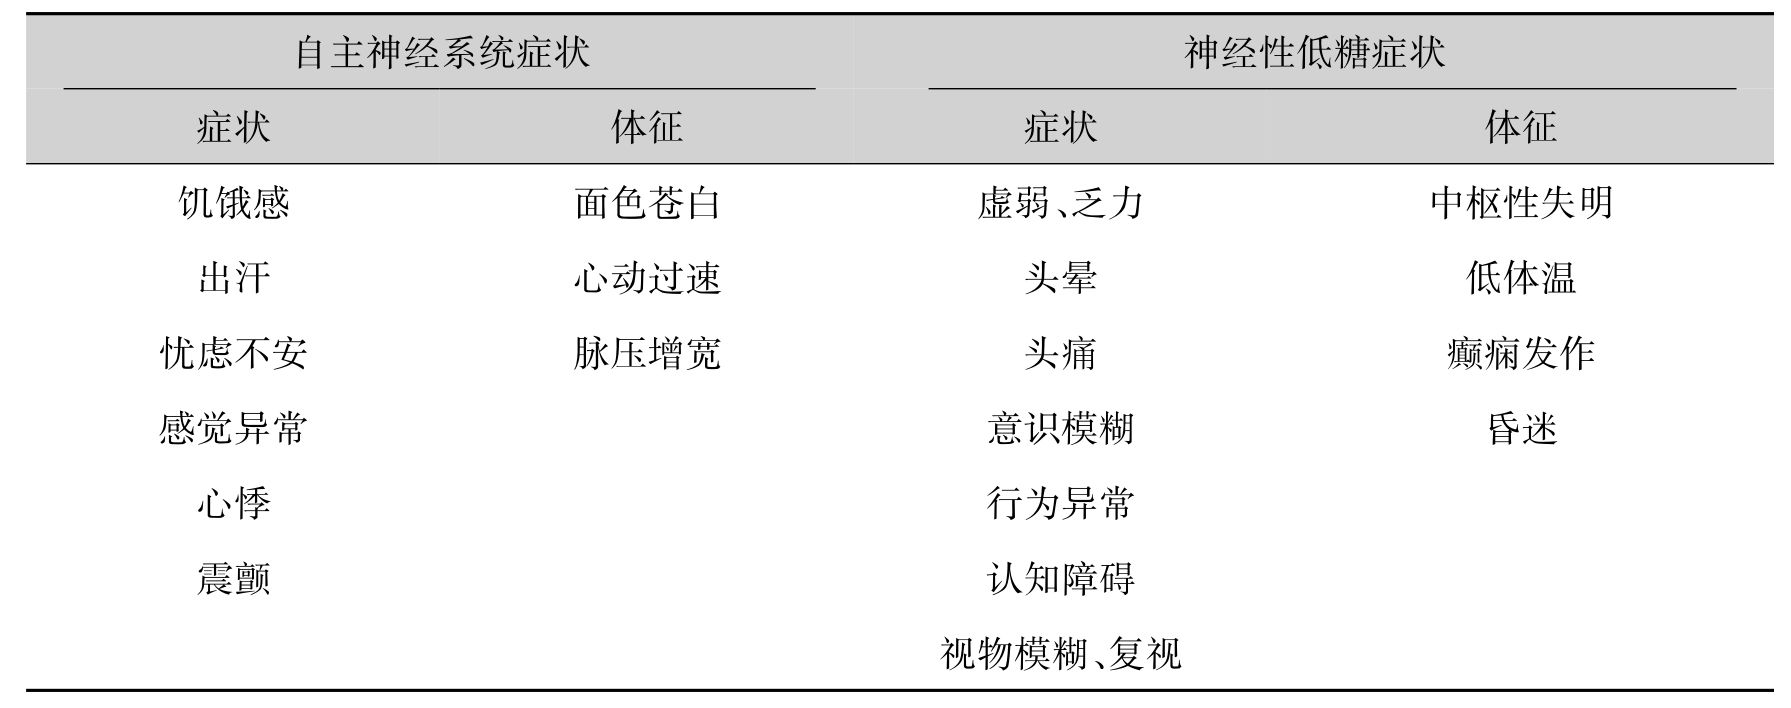
\includegraphics[width=5.95833in,height=2.35417in]{./images/Image00250.jpg}
\end{table}

血糖浓度受很多生理因素的影响。例如:禁食可使血糖浓度稍下降,于48~72小时降至最低水平;运动可促使血糖降低,较易见于长时期剧烈活动后的儿童;新生儿的血糖往往偏低,老年人亦然。

低血糖症可以是暂时性、复发性或持续性。低血糖症状的轻重,与血糖值、发展快慢以及持续时间等有关。血糖值愈低,发展愈快,持续时间愈长,则症状愈明显。低血糖症的症状和体征是由于神经元缺乏葡萄糖所致,可分为两类:自主神经系统症状和神经低糖症状(表\ref{tab41-1})。前者由自主神经系统兴奋引起,伴有肾上腺髓质释放肾上腺素进入血液循环以及靶组织内交感节后神经末梢分泌去甲肾上腺素,在正常情况下,引起儿茶酚胺释放的血糖阈值高于出现神经低糖症状时的血糖水平,因此自主神经系统的症状常先出现。神经低糖症状是大脑缺乏葡萄糖所致,和其他缺氧症状鉴别较难。

引起升糖激素释放和神经低糖症状的血糖阈值是可变的,控制不良的糖尿病患者持续高血糖可使该阈值升高,反复发作低血糖的患者阈值降低。一次严重的低血糖也可削弱儿茶酚胺对以后低血糖的反应。因此,临床上反复发作低血糖的患者可能不出现低血糖警示症状,当血糖浓度降至界限阈值时,不能作出迅速反应以避免严重的神经低糖昏迷。严重持久的低血糖发作可造成神经细胞死亡,导致永久性大脑功能损伤。

引起低血糖症的疾病较多,将按表\ref{tab41-2}的顺序分别讨论。

\begin{table}[htbp]
\centering
\caption{低血糖症的病因分类}
\label{tab41-2}
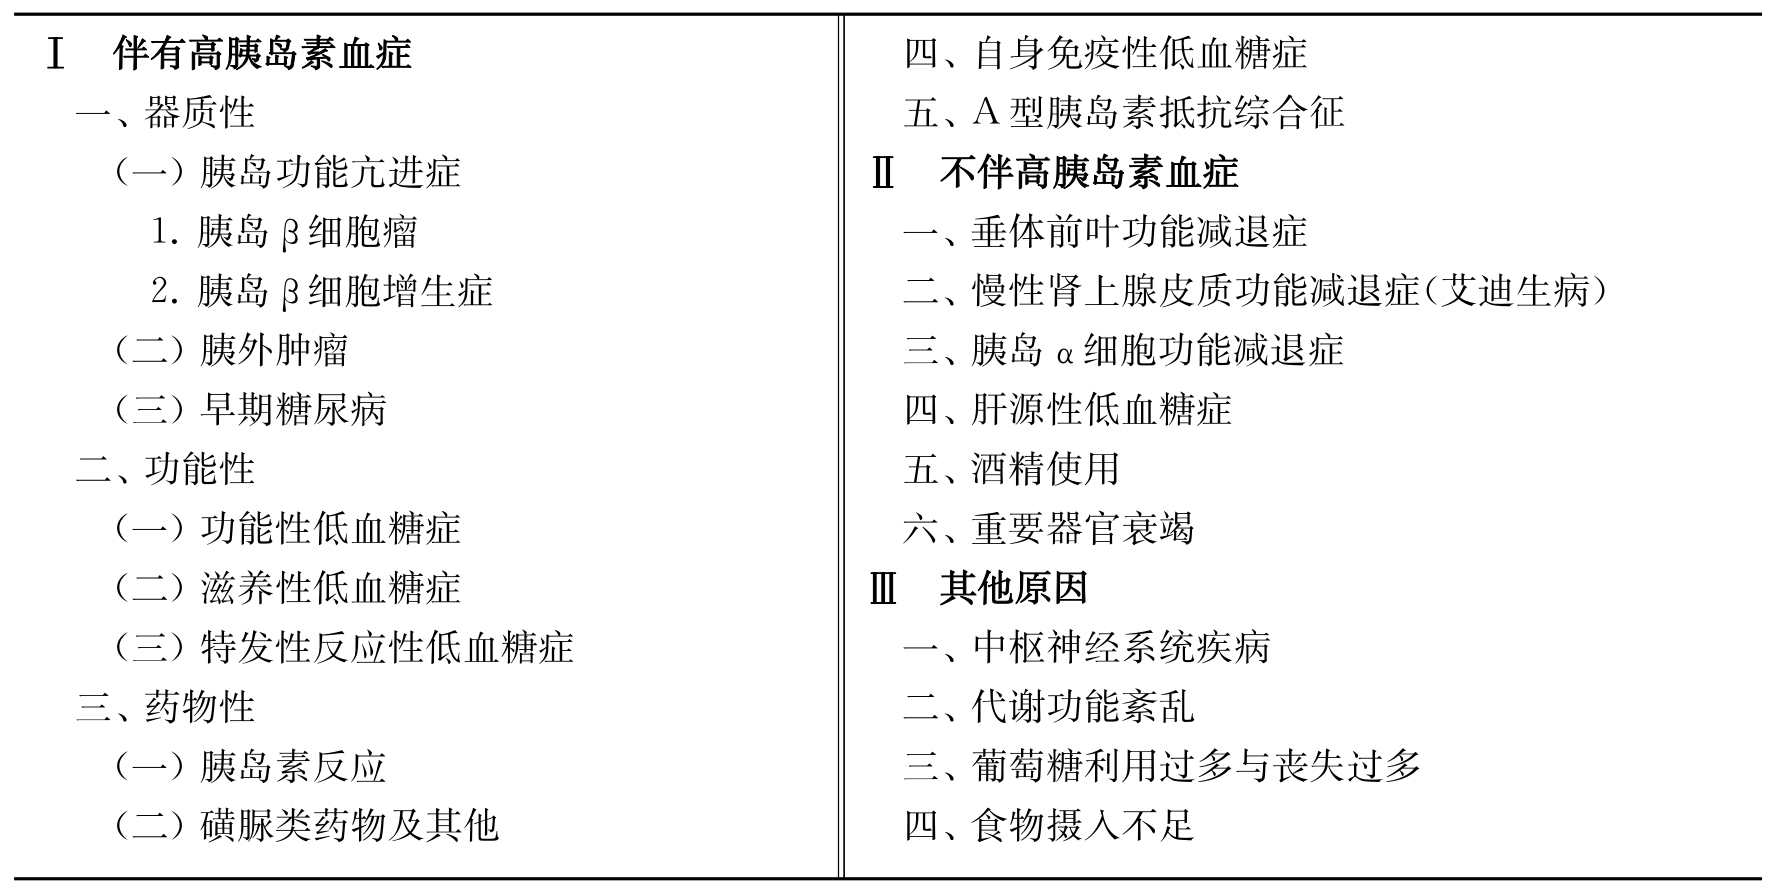
\includegraphics[width=5.90625in,height=2.95833in]{./images/Image00251.jpg}
\end{table}

\protect\hypertarget{text00318.html}{}{}

\section{136 伴有高胰岛素血症}

\subsection{136.1 器质性}

\subsubsection{一、胰岛功能亢进症(hyperinsulinism)}

\paragraph{(一)病因}

\subparagraph{1.胰岛β细胞瘤}

胰岛β细胞瘤能分泌大量胰岛素,引起严重的低血糖症,且为本病最突出的表现。此瘤约90\%为良性腺瘤,90\%为单发,90\%位于胰腺内,90\%肿瘤直径小于2cm。10\%为癌,癌所致的低血糖症更为严重。正常人胰岛组织1g可分泌胰岛素2单位,而肿瘤组织1g能分泌胰岛素多达80单位。当血糖值低于3.0mmol/L时,患者一般即出现低血糖症。胰岛β细胞瘤较少见,患病率约为0.01‰~0.04‰,男女性别无大差异,任何年龄均可发生,最年轻者为14天的婴儿,最年长者为78岁。好发于35~55岁之间。本病患者起病缓慢,症状可出现于诊断前多年,主要为反复发作性低血糖症,患者可出现出汗、震颤、心悸等自主神经症状和意识模糊、行为异常、个性改变、视物模糊,乃至昏迷等神经低糖症状。大多见于清晨早餐前,少数也可见于午、晚餐前。饥饿,劳累,精神刺激,饮酒,月经来潮,发热等可诱发低血糖症,由轻渐重,由偶发至频发,从一年仅一、二次发作渐渐增加至一日数次发作。发作时间长短不一,最短者仅3~5分钟,历时长久者可连续数日。此病确诊的重要性在于手术治疗能获根治。

\subparagraph{2.胰岛β细胞弥漫性增生症}

弥漫性胰岛β细胞增生,分泌胰岛素功能过盛,也可引起低血糖状态。国外文献报告少数病例,绝大多数为儿童,患者在餐后2~4小时出现神经低糖症状,而禁食72小时反而不出现症状。胰腺部分切除术后效果良好。胰岛β细胞增生症少见,有医院报道59年间仅见到3例,此3例均为成年患者。

\paragraph{(二)胰岛功能亢进症的诊断}

胰岛β细胞功能亢进症的诊断包括定性诊断和定位诊断。

\subparagraph{1.定性诊断}

首先要确定症状是否由低血糖引起,经典的提示胰岛β细胞功能亢进的Whipple三联症对诊断仍有重要意义,即①有发作性低血糖症状(参见表\ref{tab41-1}),空腹或体力活动可诱发发作;②空腹或发作时血糖低于2.8mmol/L;③给糖后低血糖症状随之消失。90\%的患者根据Whipple三联症可以得到正确诊断,但仍有一部分患者血糖可在正常范围,而且影响血糖的因素较多,因此,有人提出新的更为严格的四项标准:①发作时血糖<2.5mmol/L;②同时胰岛素水平≥6μU/ml;③C肽水平≥200pmol/L;④血中不含磺脲类药物。符合以上四项标准很少产生误诊。

实验室诊断有以下方法:

\hypertarget{text00318.htmlux5cux23CHP41-1-1-1-2-1-1}{}
(1)血浆胰岛素测定:

正常人血糖升高时,胰岛素分泌增多;当血糖降低至1.67mmol/L时,则胰岛素停止分泌。但在胰岛功能亢进的患者,血糖虽降低而胰岛素仍继续分泌。因此,如血糖低于1.67mmol/L而血浆胰岛素高于36~43pmol/L(5~6μU/ml)时,肯定为胰岛素不适当分泌过多。如测定胰岛素与血糖比值(血浆胰岛素U/ml,血浆葡萄糖mg/dl),则更有诊断价值。正常人此比值≤0.3,胰岛素瘤患者>0.3,甚至高达1.0或以上。但需注意的是,胰岛素水平正常并不能完全排除此病,因为并非所有胰岛素瘤患者的胰岛素水平绝对值都升高。高胰岛素原血症[即血糖<2.5mmol/L(45mg/dl)时,胰岛素原水平>20pmol/L]和胰岛素/C肽比值<1.0也有诊断意义。

\hypertarget{text00318.htmlux5cux23CHP41-1-1-1-2-1-2}{}
(2)禁食试验:

这是一种临床传统应用的筛选试验,方法简单。试验在医护人员密切观察下进行,患者只能饮白开水或清茶,每隔12小时或当症状出现时即作血糖和胰岛素测定。大多数患者不需延长至24小时即可出现典型的低血糖症状,但个别患者需延长至48~72小时,此时血糖常低于2.8mmol/L。禁食再加上运动更易诱发。不同患者甚至同一患者在不同时间做此试验可有差异。中山大学附属第一医院均曾做此试验6例,4例于禁食24小时以内诱发,另2例于禁食40小时仍未出现低血糖症状。

其他方法还有胰岛素抑制试验、甲苯磺丁脲试验和钙激发试验,可根据情况加以选用。

\subparagraph{2.定位诊断}

胰岛功能亢进的定性诊断一旦成立,即需做胰岛素瘤的定位诊断,这对手术治疗有非常重要的指导意义。由于肿瘤直径多在1~2cm,瘤内血管细小,加以胰腺周围组织结构复杂,因此虽然胰岛β细胞瘤的定位诊断方法很多,但定位诊断技术准确率报道不一,医师在选择时既要考虑到每种方法的敏感性,还要兼顾优缺点。B型超声灰阶扫描、CT扫描和MRI检查是无创性检查法,宜首先考虑应用,但超声检查的敏感性低(9\%~64\%),CT和MRI的敏感性和特异性明显高于超声,尤其是CT扫描可作为胰岛素瘤定位诊断的一线选择。当CT检查显示阴性结果而临床高度怀疑此病时需要考虑其他诊断技术的应用,如超声内镜(EUS)、选择性脾或胃十二指肠动脉造影CT(DSA)和钙剂动脉激发肝静脉采血测胰岛素检查(arterial
stimulation venous
sampling,ASVS)、术中超声探查等。这些侵入性检查方法对显示直径小于1cm的小肿瘤具有重要价值,但肿瘤的隐蔽性较强,且呈散在分布,定位较困难,定位诊断技术通常需联合使用,缺点是费用昂贵、创伤较大。中山大学附属第一医院有1例胰岛素瘤患者,为定位肿瘤,先后行了胰腺CT、MRI、DSA、腹腔镜探查以及两次超声内镜检查,第2次超声内镜检查确定了2个肿瘤,术中超声探查发现第3个肿瘤,最终成功施行了肿瘤手术切除术。

胰岛β细胞弥漫性增生症术前和术中通常无法进行定位诊断。

\paragraph{(三)鉴别诊断}

因低血糖症状出现较早,而肿瘤发现较晚,胰岛β细胞瘤的诊断有时相当困难,临床上被误诊为精神病、癔症、神经症、癫痫等,而延误多年者并不少见。中山大学附属第一医院所见7例(包括院外会诊1例),来诊前2例曾误诊为神经症达3~6年,1例误诊为癫痫达8个月,2例误诊为精神分裂症。早期诊断的关键在于提高对本病的警惕性。如患者有发作性软弱、饥饿感、颤抖、多汗以及意识丧失、精神错乱或抽搐发作,尤其是在早晨餐前或劳动后发生者,应考虑本病的可能性,并作相应的检查,以求确诊。一时无法确诊者,应继续随访及重复检查。此外,部分患者有食欲增加而致肥胖,1例19岁女性患者患病8个月,体重增加10余公斤。

胰岛β细胞瘤与慢性肾上腺皮质功能减退症都可以出现精神失常和低血糖,但前者多较肥胖,精神症状在注射葡萄糖后迅速消失;后者有明显消瘦、皮肤黏膜色素沉着、低血压,精神症状在注射葡萄糖后虽可减轻,但需用肾上腺皮质激素才能充分控制。自身免疫性低血糖症也可出现高胰岛素血症,胰岛素释放指数常显著升高,可达6.0以上,禁食试验常为阳性,与胰岛素瘤的鉴别点在于前者的患者有胰岛素注射史或含巯基药物的使用史,进餐后常有较显著的高血糖,随后出现低血糖,严重者也可发生空腹或夜间低血糖,胰腺的定位检查为阴性,胰岛素抗体或胰岛素受体抗体阳性,可伴有其他自身免疫性疾病,而后者通常表现为频发的夜间低血糖,严重者也可出现餐后低血糖,胰腺的定位检查为阳性,胰岛素抗体或胰岛素受体抗体阴性。

\subsubsection{二、胰外肿瘤}

自发性低血糖症也可见于胰腺以外的肿瘤,包括胸腔、腹腔或腹膜后发源于间质细胞的肿瘤和来源于上皮组织肿瘤。间质细胞肿瘤大多体积巨大,重量可达800~1000g,恶性程度低,生长缓慢。早期症状常表现为由于低血糖引起的大脑功能迟钝,常于饥饿时发生低血糖症,有时于餐后2~3小时发作,大多见于老年人,无性别差异。约有10\%的患者伴有内分泌疾病,如甲状腺肿大、甲状腺功能亢进症,肢端肥大症,男性乳房发育等。此组肿瘤伴低血糖症时血浆胰岛素水平一般降低。国外文献报告这类肿瘤有纤维肉瘤、间皮瘤、纤维瘤、腹腔黏液瘤等。伴有低血糖症的上皮组织肿瘤有肝细胞癌、肾上腺腺瘤或癌、胆管瘤、盲肠癌、支气管癌、肾胚胎瘤(Wilm瘤)、消化道类癌、分化差的甲状腺癌等,多于肿瘤晚期发生低血糖症。

胰外肿瘤引起低血糖的机制尚不清楚,可能原因有以下几个方面:①肿瘤产生胰岛素样物质如胰岛素样生长因子(主要为IGF-Ⅱ)、胰岛素受体抗体以及各种细胞因子等;②对内生性胰岛素过度敏感;③是由于巨大肿瘤消耗葡萄糖过多所致;④近年发现亮氨酸或异戊酸可使某些人血糖降低,有人发现巨大肿瘤中氨基酸浓度为其他组织的10倍,故认为可能是肿瘤中氨基酸进入对亮氨酸过敏患者的血流,引起低血糖症状发作。

此组病例手术割除肿瘤后低血糖症状消失。中山大学附属第一医院近年见1例肾上腺皮质癌所致的库欣综合征伴有严重低血糖,多次血糖检查微量,持续静脉滴注葡萄糖液才能维持血糖于正常水平,手术割除肿瘤重3kg;另1例为支气管癌伴有多次低血糖发作,最后因低血糖昏迷死亡。

\subsubsection{三、早期糖尿病}

部分早期2型糖尿病患者可间歇出现血糖增高及糖尿,而在餐后3~5小时常有自发性低血糖的临床表现。目前认为是由于胰腺释放胰岛素失调,进食后胰岛素分泌呈延迟而过高的反应,进食后不久血糖过高,数小时后则血糖过低。糖耐量曲线有下列特点:①空腹血糖正常或轻度升高;②第1、2小时呈高血糖水平,超过8.9mmol/L;③在3~5小时血糖突然下降可达2.8mmol/L以下,患者出现低血糖症状。此种低血糖尤需与肝源性低血糖相区别,因在重症肝脏疾病时,也可出现类似轻症糖尿病的糖耐量曲线,但后者有肝脏病病史及体征,肝功能异常,注射肾上腺素0.5~1ml及(或)胰高糖素后血糖上升不明显,可有助于鉴别。

\subsection{136.2 功能性}

\subsubsection{一、功能性低血糖症}

功能性血糖过低症也称神经源性低血糖症,主要见于一些自主神经不稳定或焦虑状态的人,是低血糖症的常见类型;由于迷走神经兴奋性过高,刺激胰岛β细胞分泌胰岛素,或β细胞对正常刺激过度反应而致自发性低血糖。高糖饮食容易引起低血糖发作。患者病史长,症状轻,绝少丧失知觉,早餐前无血糖过低,而发作常于餐后2~4小时发生,血糖值很少低至2.2mmol/L。每次发作历时约15~20分钟,随后自行恢复。此外,血糖值与症状往往不相一致,有时血糖在低值而无症状;与此相反,有时症状明显而血糖并不降低。使用镇静剂改善自主神经稳定性或口服抗胆碱药物,有时获得良好疗效。

功能性血糖过低症与肝源性低血糖症及胰岛功能亢进症(胰岛β细胞瘤或增生)的鉴别,可参考表\ref{tab41-3}。

\begin{longtable}{c}
 \caption{功能性低血糖症、肝源性低血糖症与胰岛功能亢进症的鉴别}
 \label{tab41-3}
 \endfirsthead
 \caption[]{功能性低血糖症、肝源性低血糖症与胰岛功能亢进症的鉴别}
 \endhead
 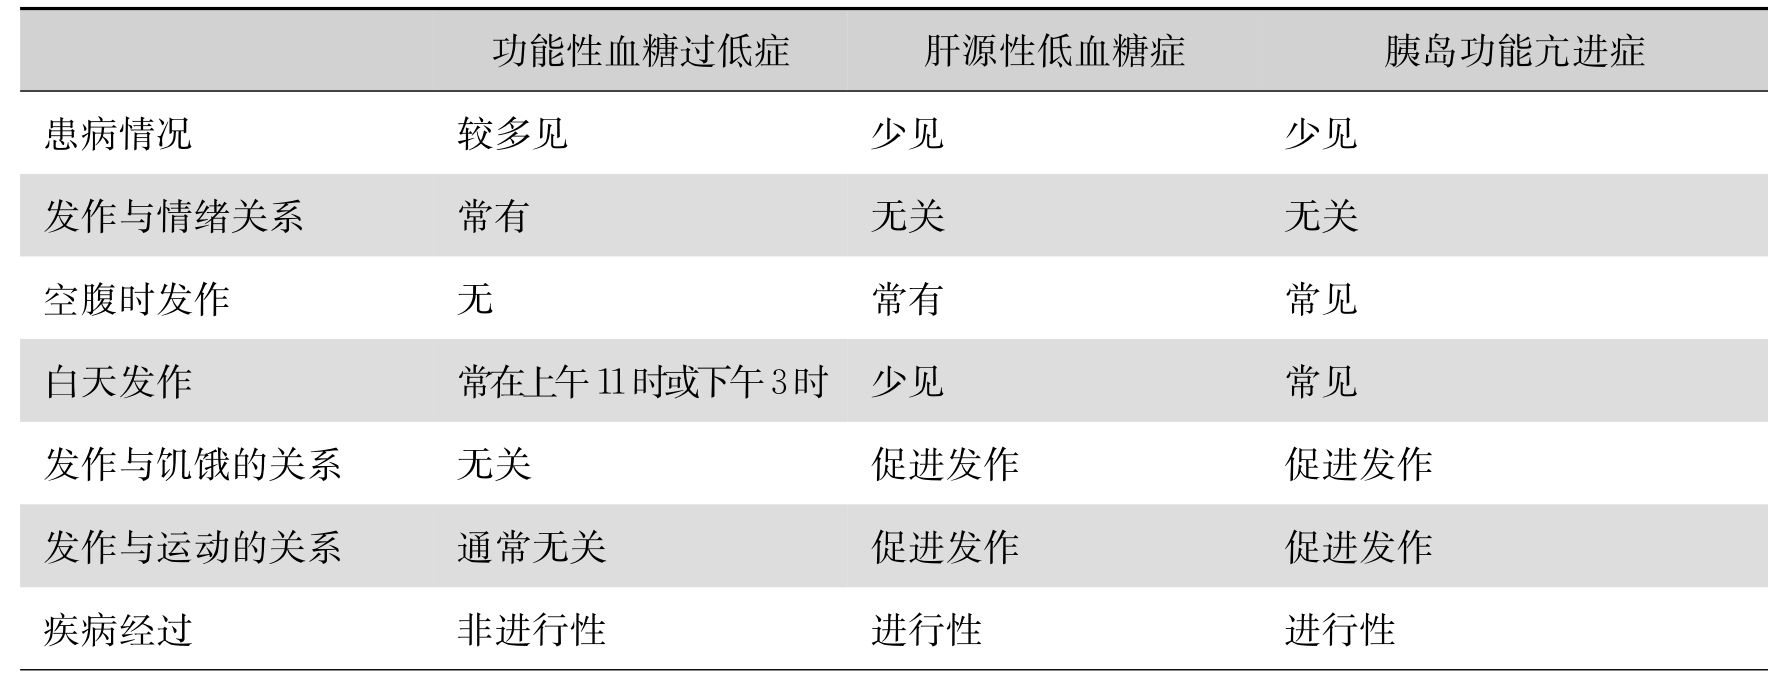
\includegraphics[width=\textwidth,height=\textheight,keepaspectratio]{./images/Image00252.jpg}\\
 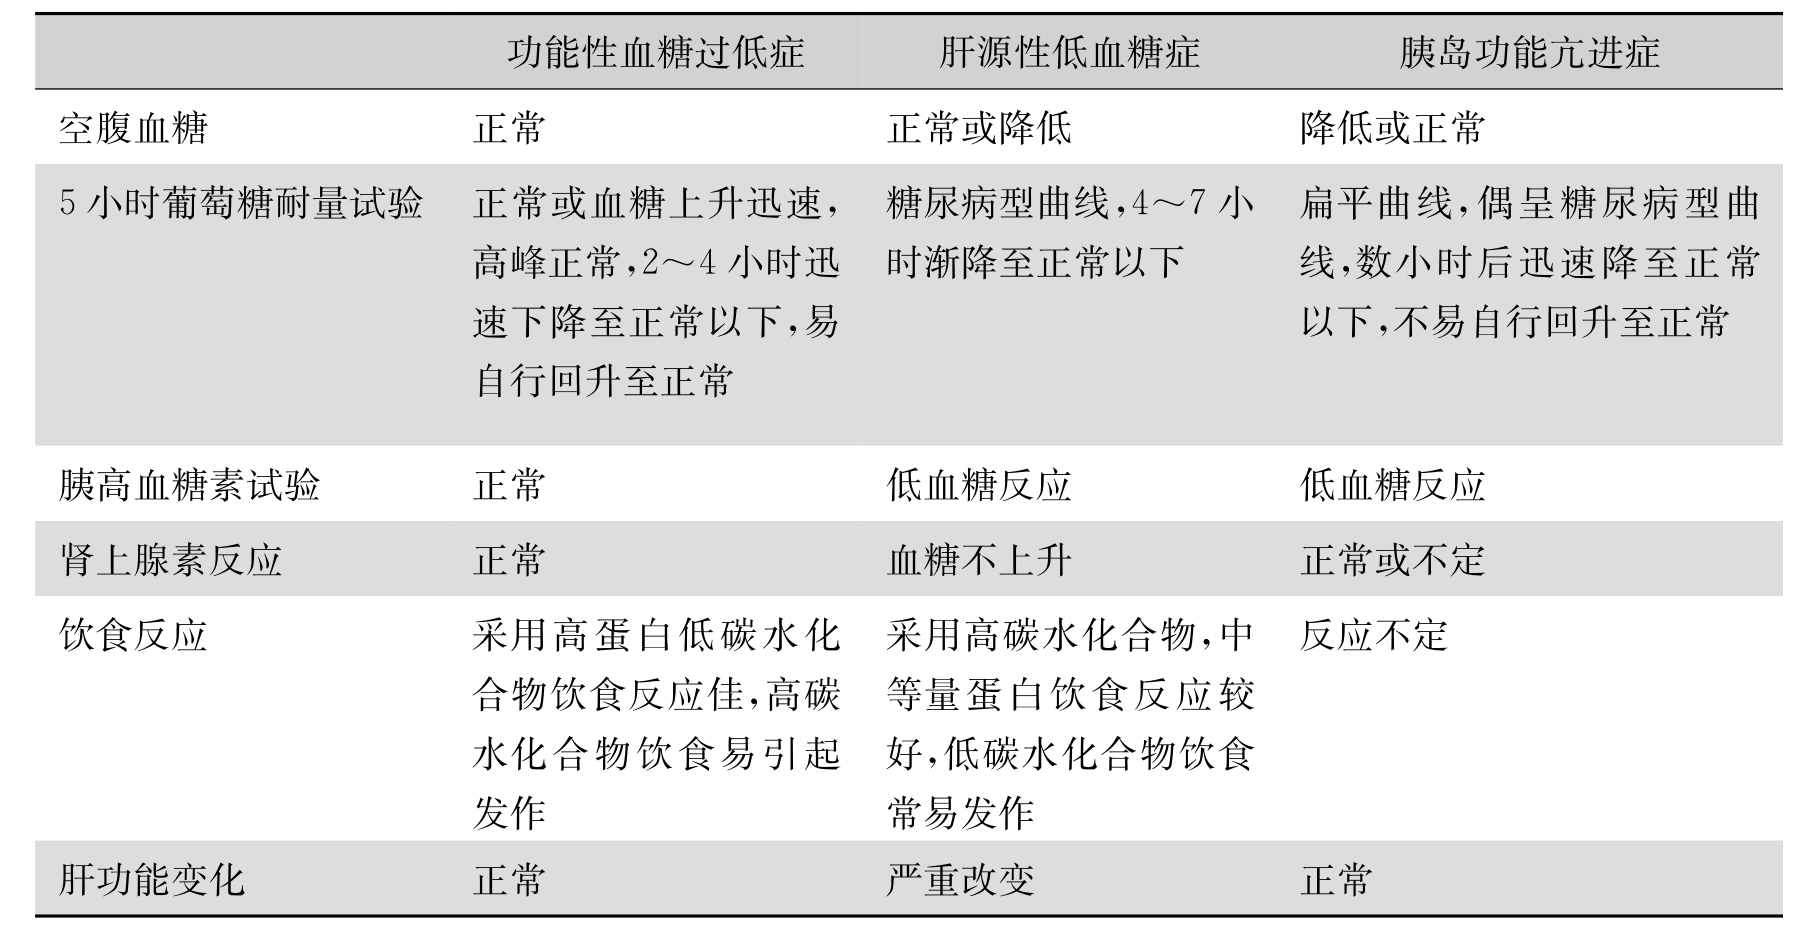
\includegraphics[width=\textwidth,height=\textheight,keepaspectratio]{./images/Image00253.jpg}
 \end{longtable}

\subsubsection{二、滋养性低血糖症}

约见于5\%~10\%胃大部分切除术后或胃空肠吻合术后患者。由于进食后胃排空过快,胃内容物迅速进入吸收面积大的肠腔,葡萄糖迅速吸收入血,使血糖急剧升高,约于30~60分钟内达高峰,刺激胰岛素过量释放,而于餐后2小时后出现低血糖症状。血糖降低程度一般较轻,常能自行缓解。

\subsubsection{三、特发性反应性低血糖症}

特发性反应性低血糖症极为罕见。患者每餐后动脉(或毛细血管)血糖均小于2.8mmol/L,其病因不明。胰岛素神经内分泌调节失常、肠道分泌GLP-1过多、胰岛素敏感性增加和胰高糖素反应削弱等解释都待进一步研究证实。

\subsection{136.3 药物性}

\subsubsection{一、胰岛素反应}

胰岛素治疗的糖尿病患者发生低血糖症是低血糖症的主要原因之一。特别是在强化治疗过程中发生率最高。在胰岛素治疗的患者中,食物量不足或者某一餐未进食、运动时以及不慎或故意的胰岛素过量是造成低血糖症常见诱因。大多1型糖尿病患者存在胰高血糖素对低血糖反应缺陷,特别是长期病程、合并自主神经病变或有反复低血糖发作病史的患者,胰高糖素和肾上腺素反应都缺乏,较易发生无症状性低血糖。有不可解释的低血糖发作的1型糖尿病患者,胰岛素需要量减少可能提示合并肾上腺皮质功能不全。患者有糖尿病病史以及胰岛素注射史,诊断不难,重点在于找出诱因并及时调整治疗方案,预防低血糖症再次发生。

\subsubsection{二、磺脲类药物及其他}

任何磺脲类药物都可产生低血糖,氯磺丙脲有很长的半衰期(35小时),是很常见的致低血糖药物。老年患者,尤其肝脏或肾脏功能受损的患者特别容易发生磺脲类引起的低血糖。经过剂型改良后的缓释、控释试剂、格列奈类和格列美脲低血糖发生率相对较低。

糖尿病患者在服用苯乙双胍、水杨酸钠等药物过程中也可出现低血糖。此类药物已证实有促进胰岛素分泌、减少胰岛素降解、减少肝糖原生成或糖原异生、在缺氧情况下增进葡萄糖利用等作用,从而可引起低血糖症。这种情况较多见于年老的、较迟确诊为糖尿病的、营养较差的、伴有脑循环障碍或(及)肾、肝功能不全的糖尿病患者。

抗疟疾药奎宁和抗心律失常药奎尼丁已被证实可诱发高胰岛素血症性低血糖,β\textsubscript{2}
-受体激动剂在幼儿中使用有引起低血糖症的报道。水杨酸盐剂量大时可引起低血糖症,多见于儿童,可能与其增加胰岛素分泌,增强其他降糖药物的作用,抑制肝糖异生和脂肪分解有关。

\subsection{136.4 自身免疫性低血糖症}

\subsubsection{一、胰岛素抗体引起的低血糖症}

糖尿病患者注射胰岛素是产生循环胰岛素抗体的最常见原因,抗体可降低注射后游离胰岛素水平,导致餐后血糖水平增高,但也可以使胰岛素半衰期增加,引起注射后延迟性低血糖症。胰岛素抗体也可见于新发1型糖尿病患者胰岛素治疗前后、1型糖尿病患者亲属或其他自身免疫性疾病患者。胰岛素抗体可以是少数患者低血糖症的主要原因,大多见于日本人,可能与日本人群相关的特殊HLAⅡ类等位基因频率较高有关。低血糖症多发生于餐后,也可见于空腹,患者在进餐后葡萄糖负荷后立刻出现高血糖,2~3小时后出现低血糖症。低血糖症的严重程度变化很大,可表现为严重的神经低糖症状,出现意识错乱、认知功能障碍甚至昏迷。患者可同时伴有其他自身免疫性疾病如Graves病、系统性红斑狼疮或类风湿关节炎。文献报道半数患者曾服用含巯基药物,如甲巯咪唑、青霉胺、卡托普利或者α-硫辛酸。部分患者可能会因为服用含有蛋氨酸(蛋氨酸可在体内代谢生成含巯基的半胱氨酸)的保健品而诱发此病。干扰素α、肼屈嗪、普鲁卡因胺和异烟肼等也可产生胰岛素抗体及引起低血糖症。患者的血清胰岛素水平通常较高(>100μU/ml),C肽水平不完全受抑制,可能升高或正常,内源性胰岛素抗体可干扰胰岛素测定,因此测定方法不同可能引起结果假性升高或降低。胰岛素抗体可通过酶联免疫吸附法测得,抗体滴度水平通常较高。大部分患者可自发性缓解,少量多次进食玉米淀粉食物有助于减轻低血糖发作次数,低血糖症严重者,也可考虑使用激素治疗。

\subsubsection{二、胰岛素受体抗体引起的低血糖症}

胰岛素受体抗体引起的低血糖症多发生在女性,常有自身免疫性疾病病史。曾有报道伴有霍奇金病。有的患者首先经历严重胰岛素抵抗阶段,伴有黑棘皮并及高血糖症,而有的患者只表现为低血糖症。由于胰岛素受体抗体的生物学功能具有多样性,因此即使同一患者在不同时期表现也不相同。胰岛素受体抗体的滴度影响患者的临床表现,抗体滴度低,部分占据胰岛素受体位点,可诱发对胰岛素受体的最大刺激而导致低血糖症;抗体滴度高可增加胰岛素受体降解,使受体数目减少和功能减弱,导致胰岛素抵抗和高血糖症。患者的胰岛素水平通常较高,但C肽水平通常部分或完全受抑制,需与胰岛β细胞瘤鉴别。

\subsection{136.5 A型胰岛素抵抗综合征}

属于常染色体显性遗传的高胰岛素性低血糖症,是胰岛素受体基因突变引起的先天性严重胰岛素抵抗综合征的一种类型。患者临床表现为消瘦体型、空腹及负荷后胰岛素显著升高、高胰岛素性低血糖症、皮肤黑棘皮征、女性患者存在多囊卵巢等。Hojlund等报道一个高胰岛素性低血糖症家系,3代中10例低血糖症患者8例曾发生低血糖昏迷,所有低血糖患者均携带胰岛素受体基因第20号外显子第1174密码子杂合错义突变,氨基酸由精氨酸突变为谷氨酰胺(R1174N)。中山大学附属第一医院也报道一例A型胰岛素抵抗综合征家系,同样为该位点突变,氨基酸由精氨酸突变为色氨酸(R1174W),携带突变的先证者及其弟弟存在吸收后及夜间低血糖症,程度较轻可耐受。该位点突变引起低血糖症的原因是由于严重胰岛素抵抗,机体代偿性分泌大量胰岛素超过肝肾代谢排泄能力所致,突变携带者均表现为胰岛素与C肽比值明显升高(0.28~0.87,正常<0.1),且高胰岛素正葡萄糖钳夹试验显示突变携带者胰岛素代谢清除率(metabolic
clearance rate,MCR)显著低于正常对照。

\protect\hypertarget{text00319.html}{}{}

\section{137 不伴高胰岛素血症}

\subsection{137.1 垂体前叶功能减退症}

垂体前叶功能减退症以产后型最为多见。本病的临床类型有四种:①性腺功能减退型;②继发性黏液性水肿型;③阵发性低血糖型;④兼有两种以上的混合型。阵发性血糖降低主要由于严重的继发性肾上腺皮质功能减退及(或)甲状腺功能减退所致,见于全部病例的10\%左右,多数于空腹时发生,以低血糖型较为严重。当葡萄糖生成减少如饮酒或脓毒血症时,或葡萄糖利用增加如剧烈运动或妊娠时,可发生低血糖症。其他一些症状可以类似慢性肾上腺皮质功能减退症,但皮肤无色素沉着,较正常人苍白。

\subsection{137.2 慢性肾上腺皮质功能减退症(Addison病)}

本病的主要临床表现是色素沉着、乏力、体重减轻、低血压。约半数病例可出现低血糖症状,多发生于空腹时、早晨或餐前,有时在餐后1~2小时发生反应性低血糖症状。在胃肠功能紊乱或感染影响食欲而致食量减少时,也易诱发。患者对胰岛素敏感,血糖易于下降,同时在血糖值稍低时,约3.3mmol/L左右,即可发生显著症状。

\subsection{137.3 胰岛α细胞功能减退症}

近年来基本肯定胰高糖素是来自胰岛α细胞,其作用是提升血糖,并在正常情况下与胰岛素共同调节血糖水平。胰高糖素不足,使胰岛素的降血糖作用缺少生理拮抗而致血糖过低。本病十分罕见,临床表现酷似胰岛功能亢进症,葡萄糖耐量试验、禁食试验及甲苯磺丁脲钠试验所见均与胰岛功能亢进症相似。故当疑及胰岛功能亢进症而手术,细致探查仍未能发现胰岛β细胞瘤或细胞增生时,应考虑本病的可能性。目前本病的诊断有赖于病理检查胰腺组织α细胞/β细胞的比率较正常减低。

\subsection{137.4 肝源性低血糖症}

严重肝脏疾病如原发性肝癌、肝硬化后期、重症肝炎、重症脂肪肝、上行感染性胆管炎等,可引起低血糖症状。肝脏具有巨大的储备功能,通常有80\%以上破坏时才出现肝衰竭和糖代谢调节失常。低血糖症的发生与肝细胞内糖原合成、储存严重不足,或糖原异生能力减弱有关。低血糖多于空腹时发生。此外,肝内酶系统的先天性缺陷,例如糖原累积病(von
Gierke病),由于肝脏不易释出葡萄糖也常出现低血糖。患者生长发育迟滞,肝脏显著肿大,血胆固醇增高,且易出现酮尿;此类疾病多于幼年发病。由于病因不同,肝脏损害程度的差别,肝源性低血糖症起病有急有缓,病程长短不一。发作的共同特点为:①多见于空腹时;②饥饿、运动,应激或限制碳水化合物时易诱发;③神经低糖症状较自主神经症状明显;④随着肝脏疾病的进展,本症发作程度及频率可增加;⑤肝病好转时低血糖症可减轻或消失;⑥有肝病的症状和体征。

在肝、胆道外科手术时,须注意体内的糖原储备情况,因可在乙醚麻醉后引起血糖过低症。

\subsection{137.5 酒精诱发的低血糖症}

酒精过量可通过抑制肝糖异生诱发低血糖症。男性较女性多见,消瘦或营养不良者更为多见。酒精中毒症状与神经低糖症的表现非常相似,增加了临床鉴别诊断的困难,因此,因酒精中毒或过量就诊的患者应常规性测定血糖。大部分患者没有自主神经症状,一些慢性酗酒者可耐受较低的血糖水平而不出现神经低糖症状。酒精过量诱发低血糖症的机制主要是通过抑制糖异生:乙醇在肝脏代谢,由乙醇脱氢酶转化为乙醛,然后在醛脱氢酶的作用下转化为乙酸,这些反应过程中产生大量的自由氢离子,使还原型辅酶Ⅰ(NADH)减少而抑制了糖异生途径前体物质的代谢。此外,乙醇还可能抑制低血糖症反应中的皮质醇激素和生长激素的释放,也可能延迟胰高糖素和肾上腺素的反应。

\subsection{137.6 重要器官衰竭}

严重充血性心力衰竭患者偶尔会发生低血糖症,机制未明,可能与恶病质、缺乏糖异生底物及缺氧和淤血导致肝功能异常有关。肾功能不全,特别是终末期肾病,也可能发生低血糖症,最常见的原因为药源性低血糖症和脓毒血症,其中7\%的低血糖发作与严重营养不良有关。糖尿病患者和非糖尿病患者进行血液透析或腹膜透析时可在透析期间或透析后短时间内发生自发性低血糖症,认为可能与透析液中高糖刺激胰岛素分泌和肾脏对胰岛素的清除率下降有关。基础血糖较低和透析中未进食的患者特别容易发生低血糖症。肾衰竭发生低血糖症的机制包括糖异生底物不足,胰高糖素作用不敏感以及糖异生受抑制。糖尿病患者合并肾衰竭时发生低血糖症也可能和降糖药物或胰岛素清除率下降有关。

另外,脓毒血症时患者常发生低血糖症。可能和肝糖原耗竭、外周葡萄糖利用增加以及细胞因子刺激胰岛素分泌有关。

\protect\hypertarget{text00320.html}{}{}

\section{138 其他原因}

\subsection{一、中枢神经系统疾病}

间脑疾病、蛛网膜下腔出血、脑炎后综合征等有时可引起低血糖,通常为轻度,甚少出现低血糖症状。

\subsection{二、代谢功能紊乱}

\subsubsection{(一)荔枝病}

是在荔枝收获季节较常见的急性疾病,可见于华南盛产荔枝的地区。患者通常为儿童(4~11岁男童最多见),个别为成人。发病前均有连续多天食用大量荔枝的历史。由于多吃荔枝,患者的正常餐量大为减少,甚至有完全不进餐者,发病前夕往往不进食晚餐。一般多在清晨发病,每以出汗、肢冷、乏力、腹痛、轻泻等为前驱症状,其后突然抽搐、昏迷。体温多正常,少数于数小时后有中等度发热,血中白细胞增多,血糖可降低至25~50mg/dl,即时注射大量葡萄糖溶液有显著疗效,若不救治可于数小时内死亡。发病机制尚未明了。尸检可发现肝脂肪变性。

\subsubsection{(二)亮氨酸过敏}

亮氨酸过敏可引起低血糖,但其产生低血糖的机制尚未清楚,可能为突然使血浆内胰岛素浓度升高所致。不能耐受果糖也可导致低血糖,其时血内果糖增高,葡萄糖水平反见明显下降,可达10mg/dl,并出现低血糖的临床表现。可能为肝脏缺乏醛缩酶所致。以上情况多见于婴儿或儿童,其重要性在于及时认识这种情况并采取措施,以免经常发作损害中枢神经。

\subsection{三、葡萄糖利用过多与丧失过多}

如哺乳期妇女、肾性糖尿病、剧烈运动或长时间重体力劳动后,均可引起低血糖,但通常只见于自主神经不稳定的人和机体糖原储备不足的人。少数重度腹泻、高热或重症甲状腺功能亢进症的患者,也可出现低血糖症状。

\subsection{四、食物摄入不足}

由于某些原因,如年老衰弱、重症慢性疾病、消化道肿瘤所致的食欲下降或吞咽困难、精神病、精神性厌食等,均可因长期食物摄入不足而致发生低血糖状态。

\protect\hypertarget{text00321.html}{}{}

\section{参考文献}

1.Okabayashi T,et al.Diagnosis and management of insulinoma.World J
Gastroenterol,2013,19(6):829-837

2.刘敏,母义明,潘长玉.胰岛β细胞瘤的定位诊断.中华内分泌代谢杂志,2007,23(3):284-288

3.王战建,等.腹膜后间皮肉瘤致低血糖昏迷一例.中华内分泌代谢杂志,1998,14(1):51

4.中华医学会内分泌学分会.中国糖尿病患者低血糖管理的专家共识.中华内分泌代谢杂志,2012,28(8):619-623

5.Huang Z,et al.Hyperinsulinaemic hypoglycaemia associated with a
heterozygous missense mutation of R1174Win the insulin
receptor(IR)gene.Clin Endocrinol,2009,71(5):659-665

\protect\hypertarget{text00322.html}{}{}

